\documentclass[a4paper,12pt]{article}

%\begin{figure}[htp]
%    \centering
%    \includegraphics[width=0.75\textwidth]{}
%\end{figure}

%%%%%%%%%%%%%%%%%%%%
%%%%  PREAMBLE  %%%%
%%%%%%%%%%%%%%%%%%%%
\usepackage{float}
\usepackage[T1]{fontenc}
\usepackage[utf8]{inputenc}

\usepackage[english,italian]{babel}
\usepackage{graphicx}     % Per includere immagini
\usepackage{subcaption}   % Per utilizzare subfigure
\usepackage{hyperref}
\usepackage{indentfirst}

\hypersetup{hidelinks}

\usepackage[margin=2.5cm]{geometry}
\usepackage{minipage-marginpar}
\usepackage{fancyhdr}
\usepackage[bottom]{footmisc}
\usepackage{lastpage}

\usepackage{enumitem}
\usepackage{tabularx}

\usepackage{graphicx}

\setlength{\parindent}{0em}
\setlength{\parskip}{1em}

\fancyhead[L]{\leftmark}
\fancyhead[R]{\shortstack[r]{Versione documento: 0.01 \\ Gruppo: G24}}

\fancyfoot[C]{}
\fancyfoot[R]{\thepage/\pageref{LastPage}}

\renewcommand{\headrulewidth}{2pt}
\renewcommand{\headruleskip}{3pt}
\setlength{\headheight}{30pt}

\renewcommand{\footrulewidth}{2pt}

\setlist[itemize]{itemsep=0.25em,topsep=0pt}
\setlist[enumerate]{itemsep=0.25em,topsep=0pt,align=left}

%%%%%%%%%%%%%%%%%%%%
%%%%  DOCUMENT  %%%%
%%%%%%%%%%%%%%%%%%%%

\title{}
\author{Gruppo G24}

\begin{document}

\pagestyle{empty}

\begin{center}

    \vspace{2 cm}

    \begin{tabular*}{\textwidth}{ c @{\extracolsep{\fill}} c }
        
\includegraphics[width=0.3\textwidth]{marchio_unitrento.pdf} & \shortstack{\Large{Dipartimento di Ingegneria} \\ \Large{e Scienza dell'Informazione}}
    \end{tabular*}

    \vspace{5 cm} 
  
    \Huge \textbf{Ingegneria del software\\}
  
    \vspace{1.5 cm} 
    \Large\textsc{Documento dei requisiti\\} 
    \vspace{3 cm} 
    \Huge\textsc{Mountain Wonders\\}
    \Large{Gruppo G24}
  
    \vspace{2 cm} 
  
    \Large{Anno accademico 2023/2024}
\end{center}

\newpage
\tableofcontents

\pagestyle{fancy}
\newpage
\section{Scopo del documento}

Il presente documento riporta i class diagram del sistema MountainWonders. Lo scopo di questo documento è quello di rappresentare le classi con relative funzionalità che verranno fornite dal sito web. Verranno utilizzati:
\begin{itemize}
    \item elencare le classi
    \item fornire una rappresentazione grafica dell'interazione tra le classi
\end{itemize}
    
\newpage

\section{Elenco delle classi}
In questa sezione mostreremo e documenteremo il diagramma delle classi. Affronteremo una descrizione approfondita dei metodi e dei parametri forniti e fondamentali al fine di realizzare un sito web consono a quello che è stato presentato nei precedenti documenti. 

\subsection{Accounts}
Questo conglomerato di classi racchiude le varie tipologie di account presenti nella pagina web. Ne sono presenti 3 tipologie: 
\begin{itemize}
    \item AccountAnonimo
    \item AccountRegistrato
    \item AccountAmministratore
\end{itemize} 
Le classi AccountAmministratore e AccountRegistrato ereditano gli argomenti della classe AccountAnonimo, non sarà possibile ereditare i metodi register() e login() poiché sono esclusivi della classe AccountAnonimo.\\
Una volta effettuato il login in base alla tipologia di utente saranno presenti diverse tipologie di metodi basate sulla gerarchia dell'account.
\begin{figure}[H]
   \centering
    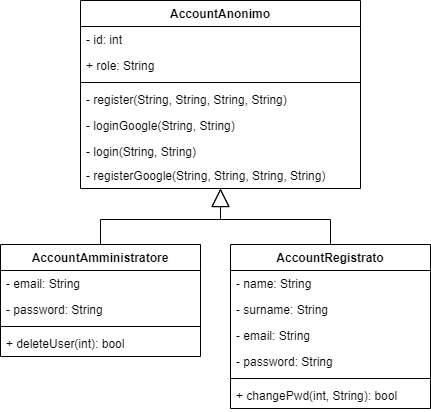
\includegraphics[width=0.6\textwidth]{D3/img/class_diagram_accounts.png}
    \caption{Class diagram accounts}
\end{figure}

\newpage
\subsection{Montagna}
Procediamo alla definizione delle classi relative alle montagne. \\
Queste due classi rappresentato: la prima la pagina web relativa alle montagne,  la seconda rappresenta l'oggetto montagna che verrà salvato all'interno del database. 
\begin{figure}[H]
   \centering
   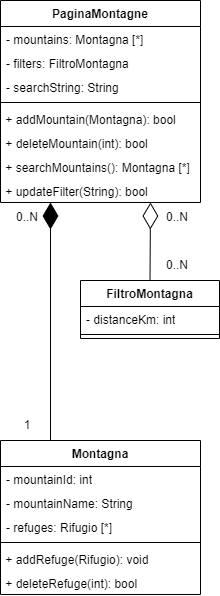
\includegraphics[width=0.25\textwidth] {D3/img/class_diagram_mountains.png}
    \caption{Class diagram montagne}
\end{figure}
\newpage
\subsection{Rifugio}
Le due classi presentate in seguito contengono una delle entità cardine del sito web: i rifugi.
\\ Nei seguenti diagrammi sono decritti gli oggetti: PaginaRifugi e Rifugio.
\\ PaginaRifugi è la classe che rappresenta la pagina web con l'elenco di tutti i rifugi (scremati se vengono applicati dei filtri oppure tutti i rifugi presenti nel database nel caso contrario). Rifugio  è la classe che contiene le informazioni di ogni singolo rifugio insieme all'insieme di recensioni che sono state effettuate per ognuno di essi.
\begin{figure}[H]
   \centering
   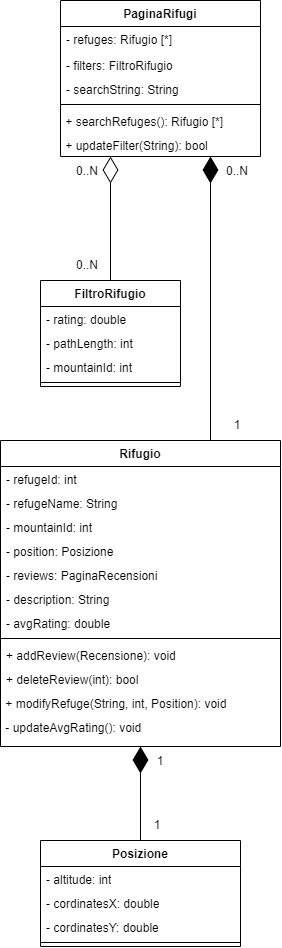
\includegraphics[width=0.25\textwidth] {D3/img/class_diagram_refuges.png}
    \caption{Class diagram rifugi}
\end{figure}
\newpage
\subsection{Recensione}
All'interno del seguente insieme vengono rappresentate le classi necessarie per gestire le recensioni.
\\ La classe PaginaRecensioni contiene e mostrerà tutte le recensioni effettuate da un utente. La classe Recensione contiene tutte le informazioni relative ad una recensione.
\begin{figure}[H]
   \centering
   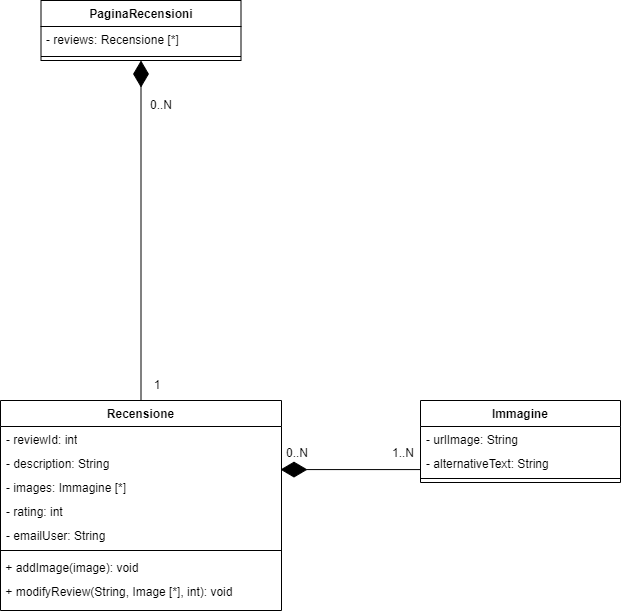
\includegraphics[width=0.5\textwidth] {D3/img/class_diagram_reviews.png}
    \caption{Class diagram rifugi}
\end{figure}

\subsection{Filtri}
All'interno del seguente insieme vengono rappresentate le classi necessarie per gestire i filtri.
\\ La classe FiltroMontagna contiene i filtri applicabili ad una montagne, mentre la classe FiltroRifugio contiene i filtri applicabili ad un rifugio.\\
Tra i filtri dei rifugi c'è anche la montagna a cui appartiene, in modo da poter mostrare tutti i rifugi di una determinata montagna.
\begin{figure}[H]
   \centering
   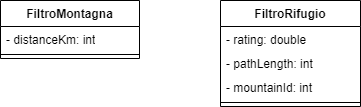
\includegraphics[width=0.5\textwidth] {D3/img/class_diagram_filters.png}
    \caption{Class diagram filtri}
\end{figure}



\newpage
\section{Diagramma classi - OCL}
In questa sezione verranno rappresentate le interazioni tra le classi utilizzando OCL (Object Contraint Language) in modo da poter descrivere concetti non rappresentabili tramite diagramma delle classi.

\subsection{PaginaMontagne}
\begin{itemize}
   \item L'addMountain() e la deleteMountain() di una montagna può essere eseguito solo se l'accesso è stato fatto dall'amministratore, la deleteMontagna() è possibile solo se sono presenti montagne e corrispondono alla montagna da eliminare. \newline \newline
   In linguaggio OCL:\newline
   \textbf{context}  PaginaMontagna::addMountain(Montagna: montagna)\newline
    \textbf{pre} AccountAnonimo.role == "Admin" \newline
    \textbf{post} : PaginaMontagna.mountains = PaginaMontagna.mountains+montagna\newline\newline
    \textbf{context}  PaginaMontagna::deleteMontagna(int: idMontagna)\newline
    \textbf{pre} PaginaMontagna.mountains != NULL and PaginaMontagna.mountains.id == idMontagna and AccountAnonimo.role == "Admin" \newline
    \textbf{post} : PaginaMontagna.mountains.id = NULL 
\end{itemize}

\subsection{Montagna}
\begin{itemize}
    \item addRefuge() è una funzionalità che può essere eseguita solo da un account registrato. \newline\newline In linguaggio OCL:\newline
    \textbf{context} Montagna::addRefuge(Rifugio: rifugio)\newline
    \textbf{pre} AccountAnonimo.role == "Registrato" \newline
    \textbf{post} Montagna.refuges= Montagna.refuges+rifugio 
    \item deleteRefuge() ha un parametro int che indica l'id del rifugio che deve essere eliminato, per questo motivo deve essere maggiore di 0, questa funzionalità è esclusiva di un ammministratore. Quando si elimina un rifugio vengono eliminate tutte le recensioni legate al rifugio. \newline\newline In linguaggio OCL:\newline
    \textbf{context} Montagna::deleteRefuge(int: idRifugio)\newline
    \textbf{pre} AccountAnonimo.role == "Admin" \newline and Montagna.refuges.refugeId == idRifugio \newline
    \textbf{post} Montagna.refuges.reviews = NULL and Montagna.refuges.refugeId = NULL 
    
    
\end{itemize}

\subsection{Rifugio}
\begin{itemize}
    \item addReview() è una funzionalità che può essere eseguita solo da un account registrato. Una volta aggiunta la recensione verrà chiamato il metodo updateAvgRating() in modo tale da aggiornare il valore precedente di avgRating. \newline \newline In linguaggio OCL:\newline
    \textbf{context} Rifugio::addReview(Recensione: recensione) \newline 
    \textbf{pre} AccountAnonimo.role == "Registrato"\newline
    \textbf{post} Rifugio.reviews = Rifugio.reviews+recensione and Rifugio::updateAvgRating() 
    \item deleteReview() è una funzionalità che può essere eseguita solo da un account registrato o amministratore e solo se esiste una recensione a cui si fa riferimento.\newline \newline In linguaggio OCL:\newline
    \textbf{context} Rifugio::deleteReview(int: idRecensione) \newline
    \textbf{pre} AccountAnonimo.role == "Registrato" \newline 
    and Recensione.reviews.reviewId==idRecensione \newline
    \textbf{post} Rifugio.reviews.reviewId = NULL  
    \item modifyRefuge() è una funzionalità esclusiva dell'amministratore, ha tre parametri che contengono i nuovi valori da assegnare agli attributi che possono essere modificati. \newline \newline In linguaggio OCL:\newline
    \textbf{context} Rifugio::modifyRefuge(String: nomeRifugio, int idMontagna, Position: posizione) \newline
    \textbf{pre} AccountAnonimo.role == "Admin" \newline
    \textbf{post} Rifugio.refugeName = nomeRifugio and Rifugio.mountainId = idMontagna and Rifugio.position=posizione 
\end{itemize}


\subsection{Recensione}
\begin{itemize}
    \item Rating recensione compreso da 1 a 5. \newline \newline In linguaggio OCL:\newline
    \textbf{context} Recensione \textbf{inv}: Recensione.rating >= 1 and Recensione.rating <= 5
     
\end{itemize}

\subsection{Posizione}
\begin{itemize}
    \item Le coordinate vengono ottenute grazie al servizio di google maps da cui è possibile selezionare la posizione di un luogo.
    \item Altitudine del rifugio compresa da 0 a 5000 metri. \newline \newline In linguaggio OCL:\newline
    \textbf{context} Posizione \textbf{inv}: Posizione.altitude >= 0 and Posizione.altitude <= 5000
\end{itemize}

\subsection{Homepage}
\begin{itemize}
    \item Nel caso in cui l'utente non abbia effettuato il login, la funzione viewUser() dell'homepage reindirizzerà l'utente nella pagina di login. \newline \newline In linguaggio OCL:\newline
    \textbf{context} AccountAnonimo.role \newline
    \textbf{pre} AccountAnonimo.role == "Anonimo"\newline
    \textbf{post} AccountAnonimo::login()\newline
    \textbf{pre} AccountAnonimo.role != "Anonimo" \newline
    \textbf{post} Homepage::viewUser()
\end{itemize}

\subsection{ChatSupporto}
\begin{itemize}
    \item Non è possibile richiedere supporto (sendRequest()) se non si è un utente registrato
    \newline \newline In linguaggio OCL:\newline
    \textbf{context} ChatSupporto.sendRequest() 
    \textbf{inv} AccountAnonimo.role == "Registrato"
    \item L'idUser è un numero maggiore di zero ed è relativo ad un account registrato. \newline \newline In linguaggio OCL:\newline
    \textbf{context} ChatSupporto
    \textbf{inv} ChatSupporto.idUser >= 1
    \item L'idRequest è un numero maggiore di zero relativo al numero identificativo della richiesta fatta dall'utente \newline \newline In linguaggio OCL:\newline
    \textbf{context} ChatSupporto
    \textbf{inv} ChatSupporto.idRequest >= 1
    \item description e answer sono degli array perché è possibile avere uno scambio di messaggi di supporto     
    \item  Una sendAnswer() può essere fatta solo da un account amministratore \newline \newline In linguaggio OCL:\newline
    \textbf{context} ChatSupporto.sendAnswer() 
    \textbf{inv} AccountAnonimo.role == "Admin"
\end{itemize}

\subsection{AccountAnonimo}
\begin{itemize}
    \item Il login può essere effettuato solo da un utente che ha già eseguito la registrazione in precedenza e quindi le sue credenziali sono già presenti all'interno del database. \newline \newline In linguaggio OCL:\newline
    \textbf{context} AccountAnonimo.login() 
    \textbf{inv} AccountAnonimo.role == "Anonimo"
    
    \item Le funzioni registerGoogle, loginGoogle vengono effettuate utilizzando le API google, i controlli vengono fatti da servizi esterni (Google).
\end{itemize}




\end{document}